\section{Determination of the cartilage subregions}
\label{sec:Subregions}
As proposed by Wirth \& Eckstein, the central weight-bearing zones of the medial / lateral femoral cartilage are divided into three subregions each (central, internal and external), while the two cartilage plates of the medial / lateral tibia are divided into five subregions each (central, internal, external, anterior, posterior). For nomenclature, refer to the table of acronyms below. 
\subsection{Determination of the femoral subregions}
Let the central weight-bearing zones be represented by two point clouds $LF'$ and $MF'$. For both central weight-bearing zones, each subregion should encompass approximately 33\% of the surface. This was achieved in practice by splitting the zones into three parts along the y-axis; two splitting points $p_1, p_2$ are chosen arbitrarily, such that $\min_{y} LF'/MF' < p_1 < p_2 < max_{y} LF'/MF', p_1 = \frac{\max_{y} LF'/MF' - \min_{y} LF'/MF'}{3}, p_2 = 2 \cdot p_1$. $p_1$ and $p_2$ are then iteratively moved along the y-axis until the constraint is satisfied, i.e. 33\% of all data points lie left of $p_1$, 33\% lie between $p_1$ and $p_2$ and 33\% lie right of $p_2$.
\begin{algorithm}
	\caption{Determination of central weight-bearing subregions}
	\label{algo:cwbzRegions}
	\begin{algorithmic}[1]
		\Procedure{CWBZRegions}{P}
		\State $P \gets \text{point cloud}$
		\State $p_1 \gets (\max_{y} P - \min_{y} P) / 3$
		\State $p_2 \gets p_1 \cdot 2$
		\State $P_1 \gets \{\:(x,y,z) \in P' \subset P \:|\: y < p_1\:\}$
		\State $P_2 \gets \{\:(x,y,z) \in P' \subset P \:|\: p_1 < y < p_2\:\}$
		\State $P_3 \gets \{\:(x,y,z) \in P' \subset P \:|\: p_2 < y\:\}$
		\Repeat
			\If{$\lvert P_1 \rvert \div \lvert P \rvert > .33$}
				\State $p_1 \gets p_1 - 1$
			\Else
				\State $p_1 \gets p_1 + 1$
			\EndIf
			\If{$\lvert P_2 \rvert \div \lvert P \rvert > .33$}
				\State $p_2 \gets p_2 - 1$
			\Else
				\State $p_2 \gets p_2 + 1$
			\EndIf
			\State $P_1 \gets \{\:(x,y,z) \in P' \subset P \:|\: y < p_1\:\}$
			\State $P_2 \gets \{\:(x,y,z) \in P' \subset P \:|\: p_1 < y < p_2\:\}$
			\State $P_3 \gets \{\:(x,y,z) \in P' \subset P \:|\: p_2 < y\:\}$
		\Until{$\lvert P_1 \rvert \approx \lvert P_2 \rvert \approx \lvert P_3 \rvert$}
		\State
		\Return $p_1, p_2$
		\EndProcedure
	\end{algorithmic}
\end{algorithm}
\subsection{Determination of the tibial subregions}
As proposed by \cite{wirth2008technique}, each plate of the tibial cartilage can be divided into five subregions (central, internal, external, anterior and posterior).
For each plate, an ellipse around the centre of the plate encompassing approximately 20\% of the plate's surface, represents the central subregion, and four triangles of variable size surrounding the ellipse represent the internal, external, anterior and posterior subregions. Let the lateral / medial tibial cartilage plates be represented by two point clouds $LT$ and $MT$. For each point cloud, the centre of gravity $c$ is determined through simple K-Means-Clustering with a single cluster, i.e. the mean of all data points of the point cloud. Two ellipses around the centres of gravity are defined as $E_L = (c_T, r_T)$ and $E_M = (c_M, r_M)$, where $c_x$ is the centre and $r_x$ is the radius of the ellipse. The ellipse therefore defines a subset of the respective cartilage plate, such that $E_x \subset xT, E_x := \{\:(x,y,z) \in E_x \:|\: \norm{(x,y,z) - c_x} \leq r_x\:\}, \lvert E_x \rvert \div \lvert xT \rvert \approx .20$. The four triangles surrounding the ellipse are determined by determining the corners $a, b, c, d$ of the plate, and data points $p \in xT$ are assigned to subregions according to their position relative to the vectors $\vec{ac}$ and $\vec{db}$, which is calculated via cross product.
\begin{algorithm}
	\caption{Determination of tibial subregions}
	\label{algo:tibialRegions}
	\begin{algorithmic}[1]
		\Procedure{TibialRegions}{P}
		\State $P \gets \text{point cloud}$
		\State $c \gets centre(P)$
		\State $r \gets \text{random initialization of radius}$
		\State $P' \gets \{\:(x,y,z) \in P' \subset P \:|\: \norm{(x,y,z) - c} \leq r\}$
		\Repeat
			\If{$\lvert P' \rvert / \lvert P \rvert > .2$}
				\State $r \gets r / 2$
			\Else
				\State $r \gets r + .5$
			\EndIf
			\State $P' \gets \{\:(x,y,z) \in P' \subset P \:|\: \norm{(x,y,z) - c} \leq r\}$
		\Until{$\lvert P' \rvert / \lvert P \rvert \approx .2$}
		\State $a \gets (\min_{x} P, \min_{y} P)$
		\State $b \gets (\max_{x} P, \min_{y} P)$
		\State $c \gets (\max_{x} P, \max_{y} P)$
		\State $d \gets (\min_{x} P, \max_{y} P)$
		\State $ac \gets c - a$
		\State $db \gets b - d$
		\State $P_a \gets \{\:(x,y,z) \in P \:|\: ac \times (c - xy)  < 0 \land db \times (b - xy) > 0\:\}$
		\State $P_p \gets \{\:(x,y,z) \in P \:|\: ac \times (c - xy)  > 0 \land db \times (b - xy) < 0\:\}$
		\State $P_i \gets \{\:(x,y,z) \in P \:|\: ac \times (c - xy)  > 0 \land db \times (b - xy) > 0\:\}$ \Comment{assuming medial}
		\State $P_a \gets \{\:(x,y,z) \in P \:|\: ac \times (c - xy)  < 0 \land db \times (b - xy) < 0\:\}$ \Comment{vice versa for lateral}
		\EndProcedure
	\end{algorithmic}
\end{algorithm}
\begin{figure}[]
	\centering
	\includegraphics[width=\linewidth]{./figures/cwbz_subregions}
	\caption{Subregions of the central weight-bearing zones of the femoral cartilage. Color codes are as follows: red - external; green - central; cyan - internal of the lateral zone; blue - internal of the medial zone}
	\label{fig:cwbz_subregions}
\end{figure}
\begin{figure}[]
	\centering
	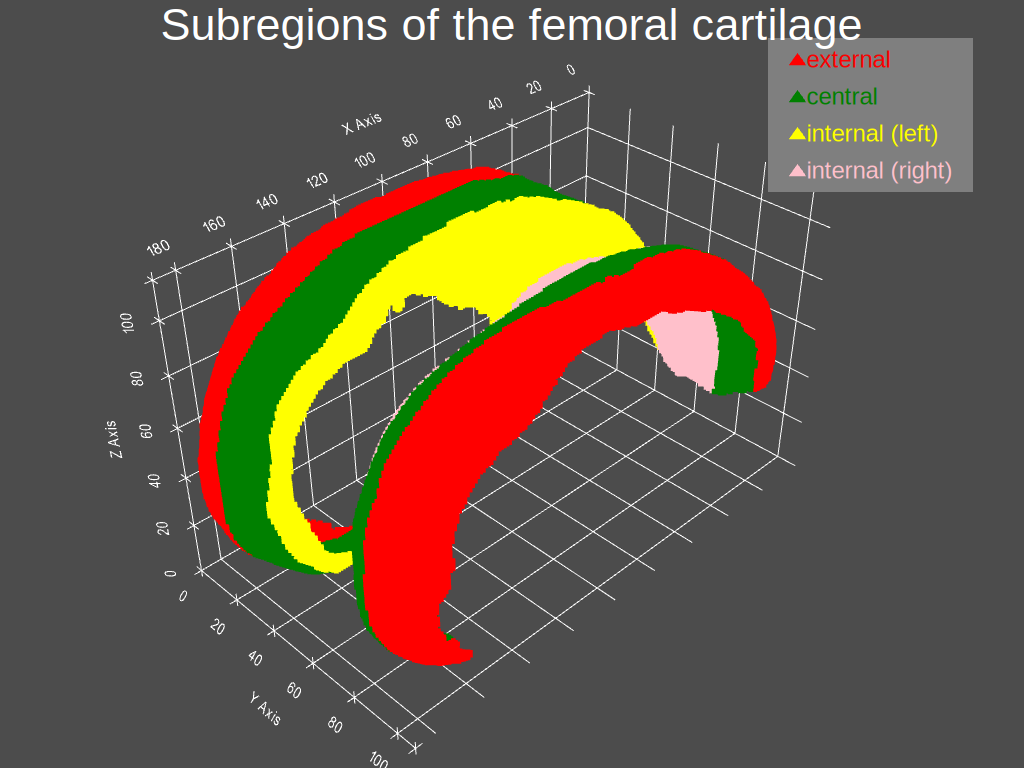
\includegraphics[width=\linewidth]{./figures/femoral_subregions}
	\caption{Subregions of the femoral cartilage. Color codes are as follows: red - lateral anterior; green - medial anterior; orange - lateral central; cyan - medial central; purple - lateral posterior; yellow - medial posterior}
	\label{fig:femoral_subregions}
\end{figure}
\begin{figure}[]
	\centering
	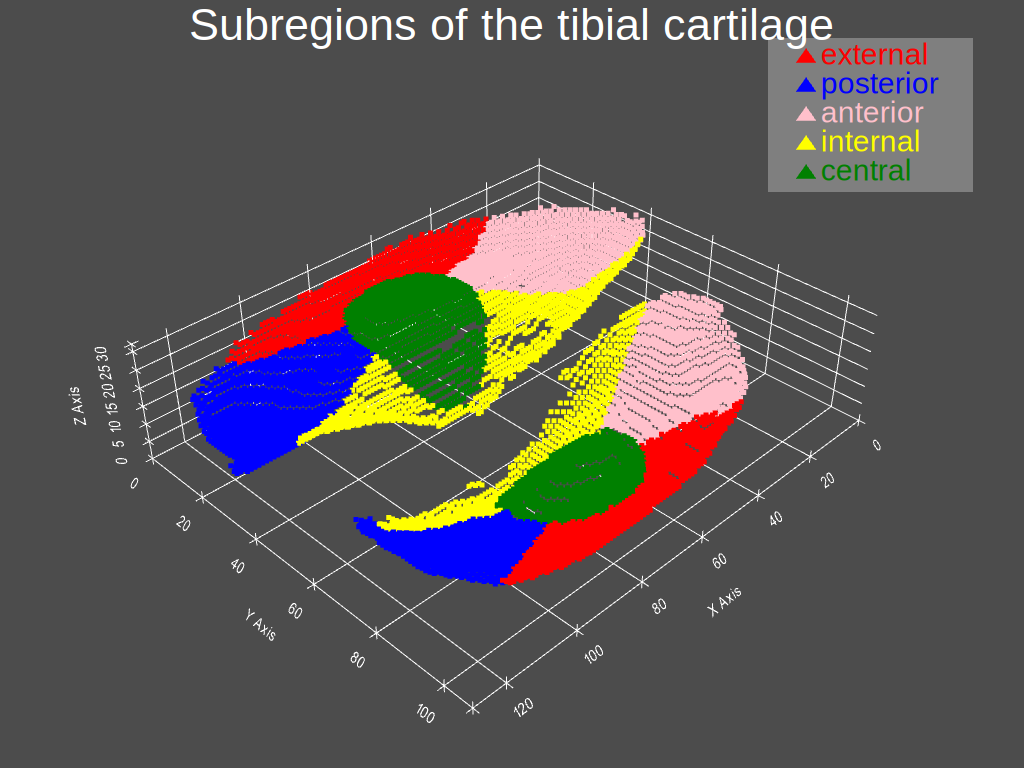
\includegraphics[width=\linewidth]{./figures/tibial_subregions}
	\caption{Subregions of the tibial cartilage. Color codes are as follows: red - internal; green - anterior; orange - posterior; blue - external; pink - central}
	\label{fig:tibial_subregions}
\end{figure}